\chapter{Background} \label{chap2}
\renewcommand{\headrulewidth}{0pt}
\lhead[\thepage]{\leftmark}
\rhead[\leftmark]{\thepage}
\cfoot[]{}

\section{Air pollution}
\subsection{Introduction}

Air pollution stands as a critical environmental issue, significantly impacting human health, ecosystems, and climate patterns. According to the World Health Organization (WHO) in 2020, approximately seven million deaths worldwide were attributed to air pollution \citep{who2020world}. Air pollutants such as nitrogen oxides (NO\textsubscript{x} = NO + NO\textsubscript{2}), carbon moNO\textsubscript{x}ide (CO), ground-level ozone (O\textsubscript{3}), sulfur dioxide (SO2) and particulate matter (PM), are directly emitted from natural or anthropogenic activities or through atmospheric photochemical reactions. Some of these pollutants are emitted alongside carbon dioxide (CO\textsubscript{2}) through combustion processes, while others are also short-lived climate forcer having direct or indirect effects on climate change by modulating global radiation budget \citep{RN3}. In addition, ozone can detrimentally impact crop yield, potentially posing future challenges to food security \citep{avnery2011global, avnery2011global2, chuwah2015global, tai2017impacts}.\par
Nitrogen dioxide (NO\textsubscript{2}) emerges as a particularly concerning pollutant due to its adverse effects on human health \citep{hamra2015lung}. Short-term exposure to elevated NO\textsubscript{2} concentrations can cause airway inflammation, increased susceptibility to respiratory infections and allergies, and aggravate existing lung or heart conditions \citep{bono2016air, kelly2011air}. Moreover, NO\textsubscript{x} lead to environmental changes by altering soil chemistry and biodiversity through nitrogen deposition via dry and wet processes \citep{bobbink2010global}. Additionally, NO\textsubscript{x} serves as a crucial precursor to tropospheric ozone (O\textsubscript{3}), along with volatile organic compounds (VOCs) \citep{akimoto2022rethinking}. NO\textsubscript{x}, CO and non-methane volatile organic compounds (NMVOCs) have an influence on the methane (CH\textsubscript{4}) lifetime by affecting the atmospheric mixing ratio of hydroxyl radicals (OH) \citep{akimoto2022rethinking}, which act as a primary sink for CH\textsubscript{4} \citep{turner2019interpreting}. Both O\textsubscript{3} and CH\textsubscript{4} are short-lived climate pollutants (SLCPs) that contribute to positive radiative forcing, thereby intensifying global warming \citep{akimoto2022rethinking}. 
Global NO\textsubscript{x} emissions predominantly stem from fossil fuel combustion within energy, industry and transportation sectors. In 2017, nearly 60\% of global NO\textsubscript{x} emissions were attributed to the energy generation (22\%), industry (15\%), and on-road transportation (23\%) sectors. These sectors notably contributed to emissions from coal combustion, especially in the energy and industry sectors (accounting for over 46\% of the emissions). Additionally, emissions from the combined combustion of liquid fuels (oil) and natural gas constituted 100\% of on-road NO\textsubscript{x} emissions \citep{mcduffie2020global}. Considering historical emissions from 1970 to 2017 recorded in the CEDS database  \citep{mcduffie2020global}, global NO\textsubscript{x} emissions reached their peak between 2011 and 2013, followed by a subsequent 7\% decrease by 2017. This reduction was primarily due to stricter emission standards phased in across North America and Europe since 1992 and in China since 2013 \citep{mcduffie2020global, zheng2018trends}. However, during the same period, global NO\textsubscript{x} emissions from the energy and industry sectors increased significantly, almost six-fold between 1970 and 2011. This surge was largely driven by regional increments in China, India, the Other Asia/Pacific region, and several African countries. The subsequent decline in emissions between 2011 and 2017 was primarily due to stringent emission control policies in China, particularly targeting coal-fired power plants and industrial coal use \citep{zheng2018trends, liu2015reduced}. Additionally, global emissions of NO\textsubscript{x} from waste combustion and agricultural activities rose by 2\% and 65\%, respectively, between 1970 and 2017. These increments contributed significantly to offsetting the recent reductions in emissions from regulated combustion sources \citep{mcduffie2020global}. \par

\subsection{Impact of weather variations on air pollution changes}

Air pollution is not solely determined by emissions but also by meteorological conditions. The lifetime of NO\textsubscript{2} is strongly influenced by meteorological parameters and photochemical reactions \citep{barre2021estimating} and varies seasonally \citep{dragomir2015modeling,kendrick2015diurnal}. During winter, photochemical reaction activity is reduced, resulting in a longer lifetime of the NO\textsubscript{2}. Additionally, seasonal variations in NO\textsubscript{2} concentration are controlled by dispersion processes which are significantly affected by changes in boundary layer height (BLH), wind speed and direction patterns due to temperature inversions in summer and winter \citep{barre2021estimating,kendrick2015diurnal}. Furthermore, seasonal variations of ozone are also influenced by meteorological conditions. The study in China showed that research conducted in China highlighted the seasonal dependence of maximum daily O\textsubscript{3} concentrations on ambient temperature rather than solar radiation during spring and summer. Conversely, autumn and winter witnessed solar radiation playing a more crucial role in determining O\textsubscript{3} levels. Wind speed exhibited a weak negative correlation with atmospheric O\textsubscript{3} levels in spring, summer, and autumn but a weak positive correlation in winter. Moisture levels in spring and autumn also impact O\textsubscript{3} concentrations due to the compensation between water vapor and O\textsubscript{3}. Higher humidity levels stimulate OH radical, elevating O\textsubscript{3} concentration in the areas with high NO\textsubscript{x}. Simultaneously, increased water vapor leads to the consumption of excited oxygen atoms, intensifying O\textsubscript{3} loss \citep{yu2021review}. \par
Over the years, Japan has implemented comprehensive measures targeting emissions from both stationary and mobile sources, leading to substantial improvements in air quality since the 1950s. examining air pollution trends from 1970 to 2018 in Japan has shed light on the interplay between these measures and pollution levels \citep{ito202130, kannari2013thirty, wakamatsu2013air}. Findings from these studies have underscored a consistent decline in the concentrations of PM2.5, NO\textsubscript{2} and SO2, indicating the direct effectiveness of human-induced emission control strategies in mitigating pollution levels. This reduction in pollutant concentrations aligns with specific actions taken to address emissions. For instance, the decline in nitrogen oxides (NO\textsubscript{x}) might be attributed to the implementation of stricter regulations governing vehicle emissions. Similarly, the reduction in sulfur dioxide (SO2) levels could be linked to the widespread adoption of marine fuels with lower sulfur content, emphasizing the direct impact of targeted interventions on pollution reduction. Nevertheless, there has been a consistent year-on-year rise in ozone concentrations across extensive areas in Japan, encompassing even rural zones unaffected by direct anthropogenic sources of air pollutants \citep{ito202130}. Previous studies highlighted the significant influence of meteorological fluctuations on ozone levels in Japan. For instance, \citep{kurokawa2009influence} highlighted the sensitivity of springtime ozone variation in Japan to outflows from continental Asia. Additionally, they found a correlation between springtime ozone and the El Nino-Southern Oscillation, indicating a relationship where higher and lower springtime ozone levels are linked to La Nina and El Nino, respectively. The summer of 2019 witnessed widespread occurrences of elevated ozone concentrations throughout Japan, as reported by \citep{fukunaga2021relationship, ito202130}.\citep{fukunaga2021relationship} proposed that the conducive conditions for elevated ozone levels during this time were attributed to clear skies and higher temperatures. They suggested that a migrating anticyclone might have carried ozone and its precursors eastward, contributing to this phenomenon. This emphasizes the importance of not only exploring the direct impact of air pollution control measures but also comprehending the role of meteorological conditions in shaping air pollution dynamics. Investigating these interdependencies could significantly enhance our ability to devise more effective measures to mitigate air pollution effectively. \par

\section{Greenhouse gas}
\subsection{Fossil fuel GHG}

Greenhouse gases (GHGs) are atmospheric gases that trap heat and contribute to warming the Earth. The major ones include carbon dioxide (CO\textsubscript{2}), methane (CH\textsubscript{4}), nitrous oxide (N2O) and Fluorinated gases (F-gases) like hydrofluorocarbons (HFCs), perfluorocarbons (PFCs), and sulfur hexafluoride (SF6). These gases persist in the atmosphere for various durations, ranging from a few years to thousands of years. They reach a well-mixed state, meaning their concentrations worldwide remain relatively consistent regardless of their sources. These gases differ significantly in their impact on atmospheric warming. To compare their effects, a metric called Global Warming Potential (GWP) was established. GWP measures how much energy emissions of a specific gas, compared to emissions of 1 ton of carbon dioxide, absorb over a given period such as 20, 100, and 500 years. A higher GWP indicates a stronger warming effect on Earth relative to carbon dioxide during that time frame. This standardized unit enables the aggregation of emissions estimates for different gases (e.g., in national GHG inventories) and assists policymakers in evaluating reduction opportunities across sectors and gases. Expressed as ‘CO\textsubscript{2} equivalent’ (CO\textsubscript{2}-e), GWP converts a gas's impact into equivalent tonnes of carbon dioxide. For instance, methane's GWP over 100 years is 27 – 29.8, signifying that one tonne of methane has a warming effect equivalent to 27 – 29.8 tonnes of CO\textsubscript{2} over a 100-year period. Furthermore, nitrous oxide (N2O) has the highest impact with GWP over 100 years is 273 \citep{RN3}. However, the amount of nitrous oxide and methane emissions have been less than that of carbon dioxide emission. \par
GHGs originate from diverse sources, encompassing both natural processes and human activities. Carbon dioxide is naturally present in the atmosphere as part of the Earth's carbon cycle, which is consistently exchanged carbon among the atmosphere, oceans, soil, plants, and animals. Human activities are altering the carbon cycle–both by adding more carbon dioxide to the atmosphere and by influencing the ability of natural sinks, like forests and soils, to remove and store carbon dioxide from the atmosphere. While carbon dioxide emissions originate from various natural sources, human-induced emissions have been primarily responsible for the substantial increase in GHGs in the atmosphere since the Industrial Revolution commenced around 1750 \citep{RN3}. In 2019, emissions included approximately 45 ± 5.5 GtCO\textsubscript{2} emissions, 11 ± 3.2 GtCO\textsubscript{2}-eq of methane (CH\textsubscript{4}), 2.7 ± 1.6 GtCO\textsubscript{2}-eq of nitrous oxide (N2O) and 1.4 ± 0.41 GtCO\textsubscript{2}-eq of fluorinated gases (F-gases) (IPCC, 2022). The primary source of carbon dioxide stems from the combustion of fossil fuels within energy conversion systems like boilers in electric power plants, engines in aircraft and automobiles, and in cooking and heating within homes and businesses, accounting for approximately 64\% of emissions. Fossil fuels also play a significant role in methane emissions, the second-largest contributor to global warming. While most GHGs originate from fossil fuel combustion, about one quarter comes from land-related activities like agriculture (mainly methane and nitrous oxide) and deforestation (mainly carbon dioxide). Additional emissions come from industrial processes (primarily carbon dioxide, nitrous oxide, and F-gases), as well as municipal waste and wastewater (mainly CH\textsubscript{4}) (IPCC, 2022). 
The estimated global net anthropogenic GHGs emissions for the year 2019 reached approximately 59 ± 6.6 GtCO\textsubscript{2}-eq, marking a 12\% increase compared to the levels seen in 2010 and a significant 54\% surge compared to the figures from 1990. Among these emissions, the dominant share and escalating growth came from CO\textsubscript{2} emissions originating from fossil fuels combustion and industrial processes (CO\textsubscript{2}-FFI), followed closely by methane emissions. Notably, the highest relative growth occurred in F-gases, albeit starting from minimal levels in 1990. During 2010–2019 period, the average annual GHG emissions surpassed those of any preceding decade on record. However, the rate of growth between 2010 and 2019 (1.3\% yr-1) was comparatively lower than that observed between 2000 and 2009 (2.1\% yr-1). In 2019, a substantial 79\% of global GHG emissions stemmed from energy, industry, transport, and building sectors combined, while 22\% originated from agriculture, forestry, and other land use (AFOLU). Global gross domestic product (GDP) per capita and population growth remained the primary drivers of CO\textsubscript{2} emissions from fossil fuel combustion throughout the last decade. The trends from 1990 continued through the years 2010-2019, with GDP per capita and population growth contributing to emissions escalation by 2.3\% yr–1 and 1.2\% yr–1, respectively. This growth outpaced the reduction in the use of energy per unit of GDP (–2\% yr –1, globally) as well as improvements in the carbon intensity of energy (–0.3\% yr –1). Therefore, emissions reductions in CO\textsubscript{2}-FFI due to improvements in energy intensity of GDP and carbon intensity of energy, have been less than emissions increase from rising global activity levels in industry, energy supply, transport, agriculture and buildings (IPCC, 2022). \par

\subsection{Terrestrial carbon fluxes}

Terrestrial ecosystems play a crucial role in mitigating global warming by serving as a persistent carbon sink, actively absorbing and storing excess carbon dioxide from the atmosphere \citep{pan2011large}. Over the period from 2010 to 2019, the terrestrial CO\textsubscript{2} sink is estimated to offset fossil CO\textsubscript{2} emissions by 35\%, surpassing the ocean, which is projected to remove 26\% of fossil-fuel-derived CO\textsubscript{2} \citep{friedlingstein2020global, wang2022disentangling}. The substantial global carbon flux, known as terrestrial gross primary production (GPP), significantly contributes to the reduction of anthropogenic CO\textsubscript{2} emissions \citep{beer2010terrestrial}. \par

\begin{figure}
    \centering
    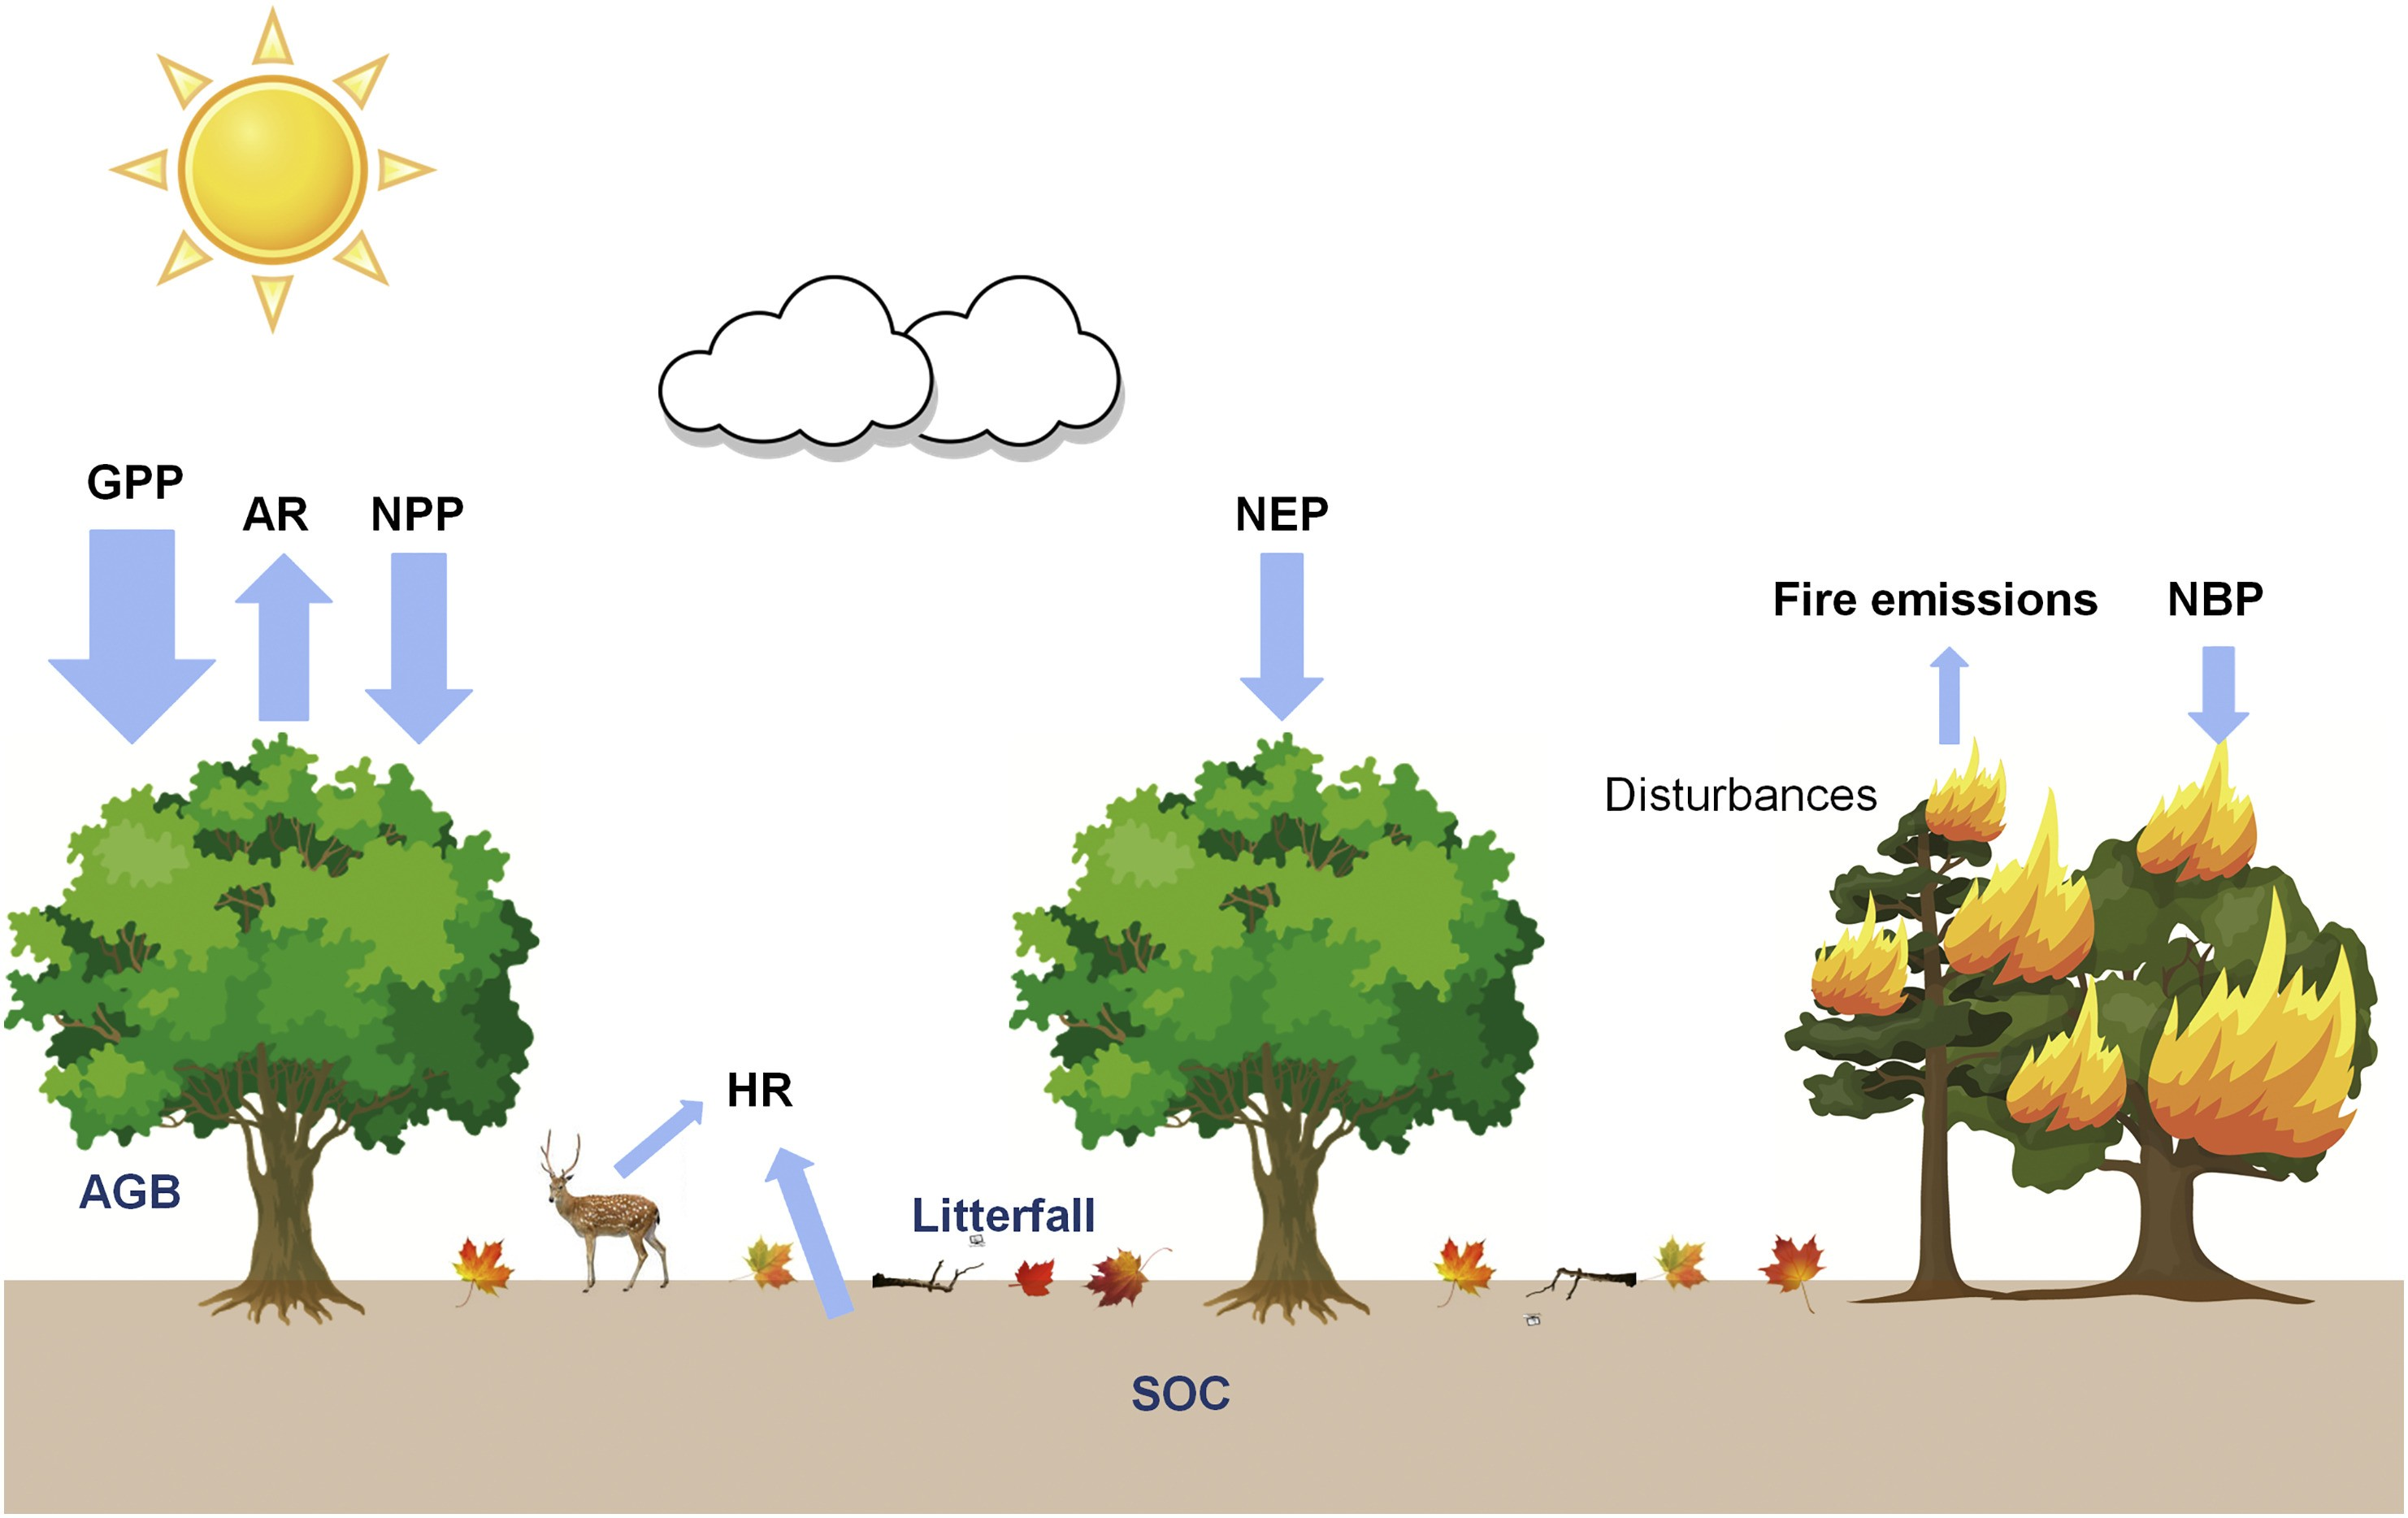
\includegraphics[width=\textwidth]{figs/chap2/fig1.jpg}
    \caption{Terrestrial carbon cycle \citep{xiao2019remote}}
    \label{chap2:fig_fig1}
\end{figure}

% need recheck
As illustrated in Figure \ref{chap2:fig_fig1}, we illustrate that Gross Primary Production (GPP) represents the total carbon sequestered by terrestrial ecosystems, serving as the foundation for food, wood, and fiber production and thereby holding significant implications for human well-being \citep{xiao2019remote}. A portion of the absorbed carbon is released back into the atmosphere through plant autotrophic respiration (AR). The disparity between GPP and AR is denoted as Net Primary Production (NPP). The material that falls to the ground from plants, such as leaves, branches, flowers, and fruits, known as litterfall, contributes to the accumulation of soil organic carbon (SOC). The size of the SOC pool is influenced by carbon inputs from litterfall and root mortality/exudation, as well as carbon release from decomposition, termed heterotrophic respiration (HR) \citep{liu2011simulating}. AR and HR collectively constitute ecosystem respiration (RECO). Net Ecosystem Production (NEP) is the absolute difference between GPP and RECO. Processes like deforestation, harvesting, and fires can result in carbon loss, with the net ecosystem carbon balance referred to as Net Biome Production (NBP). Disturbances, crucial ecosystem processes, impact carbon cycle dynamics. Wildfires, for example, lead to immediate carbon transfer from ecosystems to the atmosphere. Fires, along with other disturbances such as insect and disease outbreaks, droughts, severe storms, and harvesting, can cause substantial effects on GPP and respiration, with these impacts persisting for decades as ecosystems recover. \par

Estimating GPP involves various methods, such as simulating dynamic global vegetation models (DGVMs) like those employed in the TRENDY project \citep{sitch2015recent, le2018global}, upscaling from measurements obtained through eddy covariance (EC) flux tower and satellite observations \citep{jung2019fluxcom, zeng2020global}. However, all these approaches rely on plant functional types (PFTs) to estimate ecosystem productivity \citep{poulter2011plant, poulter2015plant, lin2021improved, guo2023estimating, yan2023integrating}. Inconsistencies in PFT maps can significantly contribute to uncertainties in GPP estimations, as well as other climate-relevant variables, at both regional and global scales \citep{poulter2011plant}. Particularly in the tropical region, the sparse distribution of EC sites, the high species richness of trees, and the complex vertical structure of tropical rainforests pose challenges \citep{montgomery2001forest}, making it difficult to accurately quantify the seasonality of carbon fluxes \citep{xu2015satellite}. \par

\section{Relationship between air pollution and greenhouse gas}
CO\textsubscript{2} is considered one of the most important GHGs, which has played a significant role in the current and future global climate change. Meanwhile, Nitrogen dioxide (NO\textsubscript{2}) emerges as a particularly concerning pollutant due to its adverse effects on human health and ecosystem. Their atmospheric concentration has considerably increased since the Industrial Revolution and is attributed mostly to anthropogenic sources, especially fossil-fuel (FF) combustion (…). While CO\textsubscript{2} emission reduction has become a goal of international agreements such as the Kyoto Protocol \citep{protocol1997united} and the Paris Agreement on Climate Change (\url{https://unfccc.int/process-and-meetings/the-paris-agreement}), the air pollution control measures reducing NO\textsubscript{2} emission have been implemented in Northern America, Europe and China to improve local air quality (…). Therefore, accurate knowledge of fossil fuel CO\textsubscript{2} and NO\textsubscript{2} emissions as well as their trends pose an importance both for climate prediction and mitigation policy purposes. \par

Fossil fuel combustion is mainly contributor of CO\textsubscript{2} and co-emitter NO\textsubscript{2} emission. These emissions are driven by activity such as fuel consumption, but differ by their relative proportion (i.e., emission factor)\citep{miyazaki2023predictability}. Global fossil fuel CO\textsubscript{2} emission inventories (e.g.  CDIAC \citep{andres2012synthesis}, ODIAC \citep{oda2011very, oda2018open}, EDGAR \citep{crippa2020high}, FFDAS \citep{asefi2014multiyear}, and CEDS \citep{hoesly2018historical}) are compiled from available national emission inventory. Fossil CO\textsubscript{2} emissions are estimated by combining economic activity data and emissions factors, with different levels of methodological complexity (tiers) or approaches (e.g., IPCC Guidelines for National Greenhouse Gas Inventories). Several organizations or groups provide estimates of fossil CO\textsubscript{2} emissions, with each dataset having slightly different system boundaries, methods, activity data, and emissions factors \citep{andrew2020comparison}. This “bottom-up” approach based on available statistical information regarding economic activities and corresponding technologies. Such error and bias information can cause the an uncertainty that is generally within ±10\% among these inventories at global scale, however, the uncertainty in emission estimates significantly varied in different countries, from 10\% in developed countries\citep{essd-11-1783-2019} but larger uncertainty in rapidly developing countries such as 8–24\% for China \citep{han2020evaluating, marland2008uncertainties} to more than 50\% for least developed countries \citep{andres2016gridded, essd-11-1783-2019, oda2018open}. For the case in China, large variations between nine emission inventories were largely due to the different emission factors related to coal quality and activity data \citep{han2020evaluating,miyazaki2023predictability}. Spatially explicit inventories depend on proxies such as population and remote sensing in order to spatially allocate country totals. Differences in these approaches can lead to large discrepancies in spatial patterns from national to global scale. Furthermore, these emissions data are mostly self-reported by national governments, which can take several years to produce \citep{marland2008uncertainties}. Air quality emission inventories, like fossil fuel CO\textsubscript{2} emission, use similar methods to determine fuel consumption and sector-based emission factors, and consequently incur substantial latency in their reporting \citep{miyazaki2023predictability}.\par

Lately, “top-down” method emerges as an additional approach to estimating fossil fuel CO\textsubscript{2} emissions for estimating fossil fuel CO\textsubscript{2} emissions, propelled by advancements in satellite observations and data assimilation frameworks. This approach leverages direct CO\textsubscript{2} observations obtained from satellite imagery to estimate CO\textsubscript{2} emissions. However, existing satellites like the Greenhouse gases Observing SATellite (GOSAT) and Orbiting Carbon Observatory-2 (OCO-2) were designed to focus on the spatiotemporal distribution of natural carbon fluxes on regional scales rather than to quantify anthropogenic emissions \citep{nassar2017quantifying, yang2023using}. Consequently, the limitations in spatial and temporal resolution of these CO\textsubscript{2} observations hinder their capacity to estimate CO\textsubscript{2} emissions at urban or city levels. \par

\begin{figure}[tbh!]
    \centering
    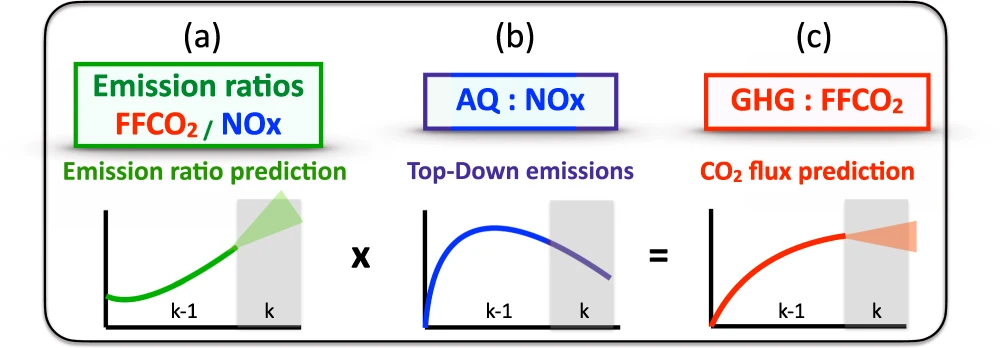
\includegraphics[width=\textwidth]{figs/chap2/aq_nox_ratio.png}
    \caption[Fossil fuel CO\textsubscript{2} prediction from top-down NO\textsubscript{x}]{Changes in CO\textsubscript{2}/NO\textsubscript{x} emission ratio for the past (t=k-1) are estimated using top-down NO\textsubscript{x} emissions and bottom-up fossil fuel CO\textsubscript{2} (FFCO\textsubscript{2}) inventories (a and b). The recent (t=k) CO\textsubscript{2}/NO\textsubscript{x} level is predicted using timeseries forecasting model based on data in the past (t=k-1) to predict (c) the CO\textsubscript{2} at the recent time (t=k) \citep{miyazaki2023predictability}.}
    \label{fig:chap2_fig2}
\end{figure}

Conversely, existing long-term satellite-derived NO\textsubscript{2} observations, such as OMI or TROPOMI, exhibit more advanced capabilities with higher resolutions in spatiotemporal aspects. They hold the potential to serve as instruments in constraining fossil fuel CO\textsubscript{2} emissions at city levels. Thus, an indirect ”top-down” method harnesses proxies like NO\textsubscript{2} observations, given their co-emission with fossil fuel CO\textsubscript{2} combustion. This indirect method proves beneficial in constraining fossil CO\textsubscript{2} emissions, monitoring their temporal fluctuations, while distinguishing them from biogenic sources of CO\textsubscript{2} emission itself \citep{ciais2014current, goldberg2019exploiting}. Satellite-based NO\textsubscript{2} observations, combined with NO\textsubscript{x}:CO\textsubscript{2} inventory ratios, have been instrumental in estimating CO\textsubscript{2} emissions indirectly. These approaches have been applied at national scales in countries such as the US, Europe, China, and India \citep{konovalov2016estimation, zheng2020satellite, miyazaki2023predictability} and at city levels, such as in Wuhan \citep{zhang2023quantifying} Buenos Aires, Melbourne, and Mexico City \citep{yang2023using}. However, such analyses have not yet been conducted either at the national or municipal levels in Japan. Conducting studies employing these methodologies both at national and cities levels in Japan could provide supplemental independent datasets. These datasets would serve to refine and evaluate "bottom-up" inventories and to assess the efficacy of current climate change mitigation strategies related to reducing fossil fuel CO\textsubscript{2} emissions, contributing insights from local to global scales. Therefore, such investigations are necessary and could offer valuable information to refine our understanding of CO\textsubscript{2} emissions and strategies for mitigating climate change. \par

\section{Air pollution, GHGs and SDGs}
\subsection{Air pollution and SDGs}
While air pollution is intricately linked to almost all other SDGs, encompassing areas such as health, water, energy, economic growth, employment, infrastructure, cities, sustainable consumption and production, climate, water, and land, its significance is not clearly emphasized in the structure of the SDGs, as noted by \citep{elder2016strengthening}. To be specific, air pollution is explicitly addressed in three goals, with one target assigned to each:
\begin{itemize}
    \item \textbf{3.9 (Health)}: By 2030, substantially reduce the number of deaths and illnesses from hazardous chemicals andair, water and soil pollution and contamination.
    \item \textbf{11.6 (Cities)}: By 2030, reduce the adverse per capita environmental impact of cities, including by payingspecial attention to air quality and municipal and other waste Management.
    \item \textbf{12.4 (Responsible consumption and production)}: By 2020, achieve the environmentally sound management of chemicals and all wastes throughout theirlifecycle, in accordance with agreed international frameworks, and significantly reduce their release toair, water and soil in order to minimize their adverse impacts on human health and the environment.
\end{itemize}

\begin{figure}[tbh!]
    \centering
    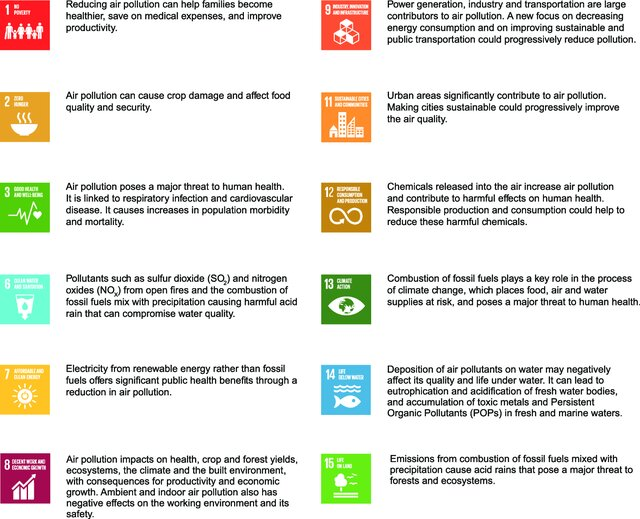
\includegraphics[width=\textwidth]{figs/chap2/How-air-pollution-relates-to-the-UN-Sustainable-Development-Goals_W640.jpg}
    \caption{How air pollution relates to the SDGs \citep{aq2017eu}}
    \label{fig:chap2_fig3}
\end{figure}
\begin{figure}[tbh!]
    \centering
    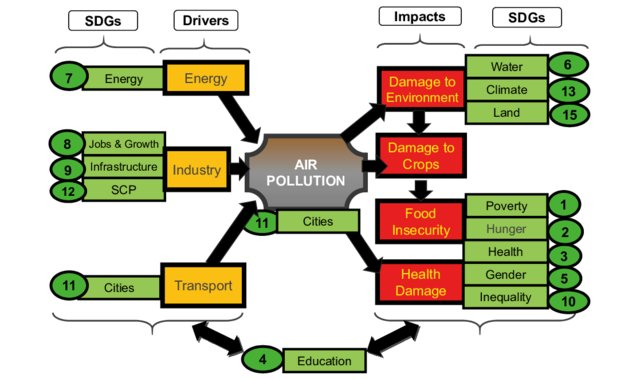
\includegraphics[width=\textwidth]{figs/chap2/Relation-of-SDGs-to-Air-Pollutions-Drivers-and-Impacts.jpg}
    \caption{Relation of SDGs to air pollution drivers and impacts \citep{elder2016strengthening}}
    \label{fig:chap2_fig4}
\end{figure}
In Figures \ref{fig:chap2_fig3} and \ref{fig:chap2_fig4}, I illustrate the connection between air pollution and the Sustainable Development Goals (SDGs) using insights from the earlier study by \citep{aq2017eu}. Additionally, I depict the relation between SDGs and the drivers and impacts of air pollution, as highlighted in the work by \citep{elder2016strengthening}. 
\begin{itemize}
    \item Goal 1 - No Poverty: Individuals and families experiencing poverty are more susceptible to the adverse effects of air pollution, particularly those reliant on outdoor labor, such as sulphur mining in active volcanoes.
    \item  Goal 2 - Zero Hunger: Air pollution has the potential to diminish crop yields and agricultural productivity, as evidenced by studies like \citep{avnery2011global}.
    \item Goal 3 - Health and Well-being: Air pollution poses a significant threat to human health \citep{who2020world}, leading to heightened morbidity and mortality rates.
    \item Goal 4 - Education: There is an expectation that educating the population will contribute to the reduction of air pollution and its future impacts.
    \item Goal 5 - Gender equality: In certain countries, women, especially those exposed to indoor air pollution from cook stoves, are more likely to bear the brunt of air pollution.
    \item Goal 6 - Water and sanitation: Pollutants like SO2 and NO\textsubscript{2}, originating from open fires and fossil fuel combustion, can mix with precipitation, resulting in harmful acid rain that compromises water quality.
    \item Goal 7 - Energy: The anticipated adoption of renewable energy is expected to significantly mitigate air pollution.
    \item Goal 8 - Economic growth: Air pollution affects health, agricultural production, and ecosystems, with repercussions for productivity and economic growth. Improving resource efficiency and decoupling economic growth from environmental degradation should contribute to reducing air pollution.
    \item Goal 9 - Infrastructure, industrialization: Power generation, industry, and transportation are major contributors to air pollution. Calls for sustainable industrialization and infrastructure, with increased resource use efficiency and the adoption of clean technologies, are expected to reduce air pollution.
    \item Goal 11 - Cities: Urban areas are significant contributors to air pollution. Making cities sustainable could progressively enhance air quality.
    \item Goal 12 - Sustainable consumption and production: Sustainable production, coupled with the removal of fossil fuel subsidies, would contribute to reducing air pollution.
    \item Goal 13 - Climate action: Simultaneously reducing greenhouse gases and air pollution requires a reduction in the combustion of fossil fuels, a key contributor to climate change.
    \item Goal 14 - Oceans: Air pollution deposition on water may affect its quality and marine life, leading to eutrophication and acidification of freshwater.
    \item Goal 15 - Biodiversity, Forest: Emissions from the combustion of fossil fuels mixed with precipitation can cause acid rain, threatening forests and ecosystems.
    \item Goal 16 - Peace: Recent armed conflicts in Ukraine and Russia, and Israel and Palestine contribute to an increase in military vehicles and weapons, causing air pollution and producing toxic dust.
\end{itemize}
\subsection{Greenhouse gas and SDGs}
GHGs are atmospheric gases that trap heat and contribute to warming the Earth causing climate change which pose a significant threat to SDGs, impacting vulnerable populations in developing and less-developed countries with intensified extreme weather events such as drought and flood, resulting in inequalities and hindering progress toward many SDGs (as shown in Figure \ref{fig:chap2_fig5}). \par
Effective action to combat climate change is articulated as the goal 13 (Climate Action), emphasizing mitigation, adaptation measures and building resilience to climate-related hazards. ctions to reduce climate risk can interact with other sustainable development objectives in positive ways (synergies) and negative ways (trade-offs) \citep{lee2023climate}. 
\begin{figure}[tbh!]
    \centering
    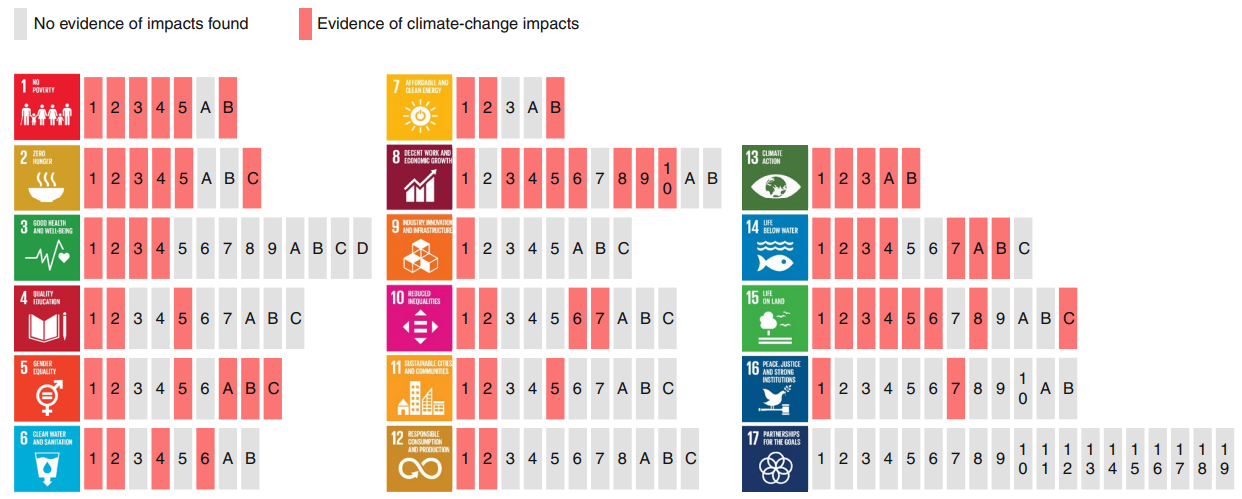
\includegraphics[width=\textwidth]{figs/chap2/impact_cc_to_sdgs.png}
    \caption{Impacts of climate change on the achievement of the SDGs \citep{fuso2019connecting}}
    \label{fig:chap2_fig5}
\end{figure}
Figure \ref{fig:chap2_fig6} illustrate the potential synergies and trade-offs between the portfolio of climate change mitigation and adaptation options and the SDGs based on the IPCC report \citep{lee2023climate}. An illustration of synergy is found in sustainable forest management, preventing deforestation emissions and sequestering carbon at a reasonable cost, aligning with various dimensions of sustainable development. For instance, it supports food security (SDG 2), clean water (SDG 6), and ecosystem protection (SDG 15). Another instance of synergy arises when climate adaptation measures, such as coastal or agricultural projects, empower women, enhancing local incomes, health, and ecosystems. \par
\begin{figure}[p]
    \centering
    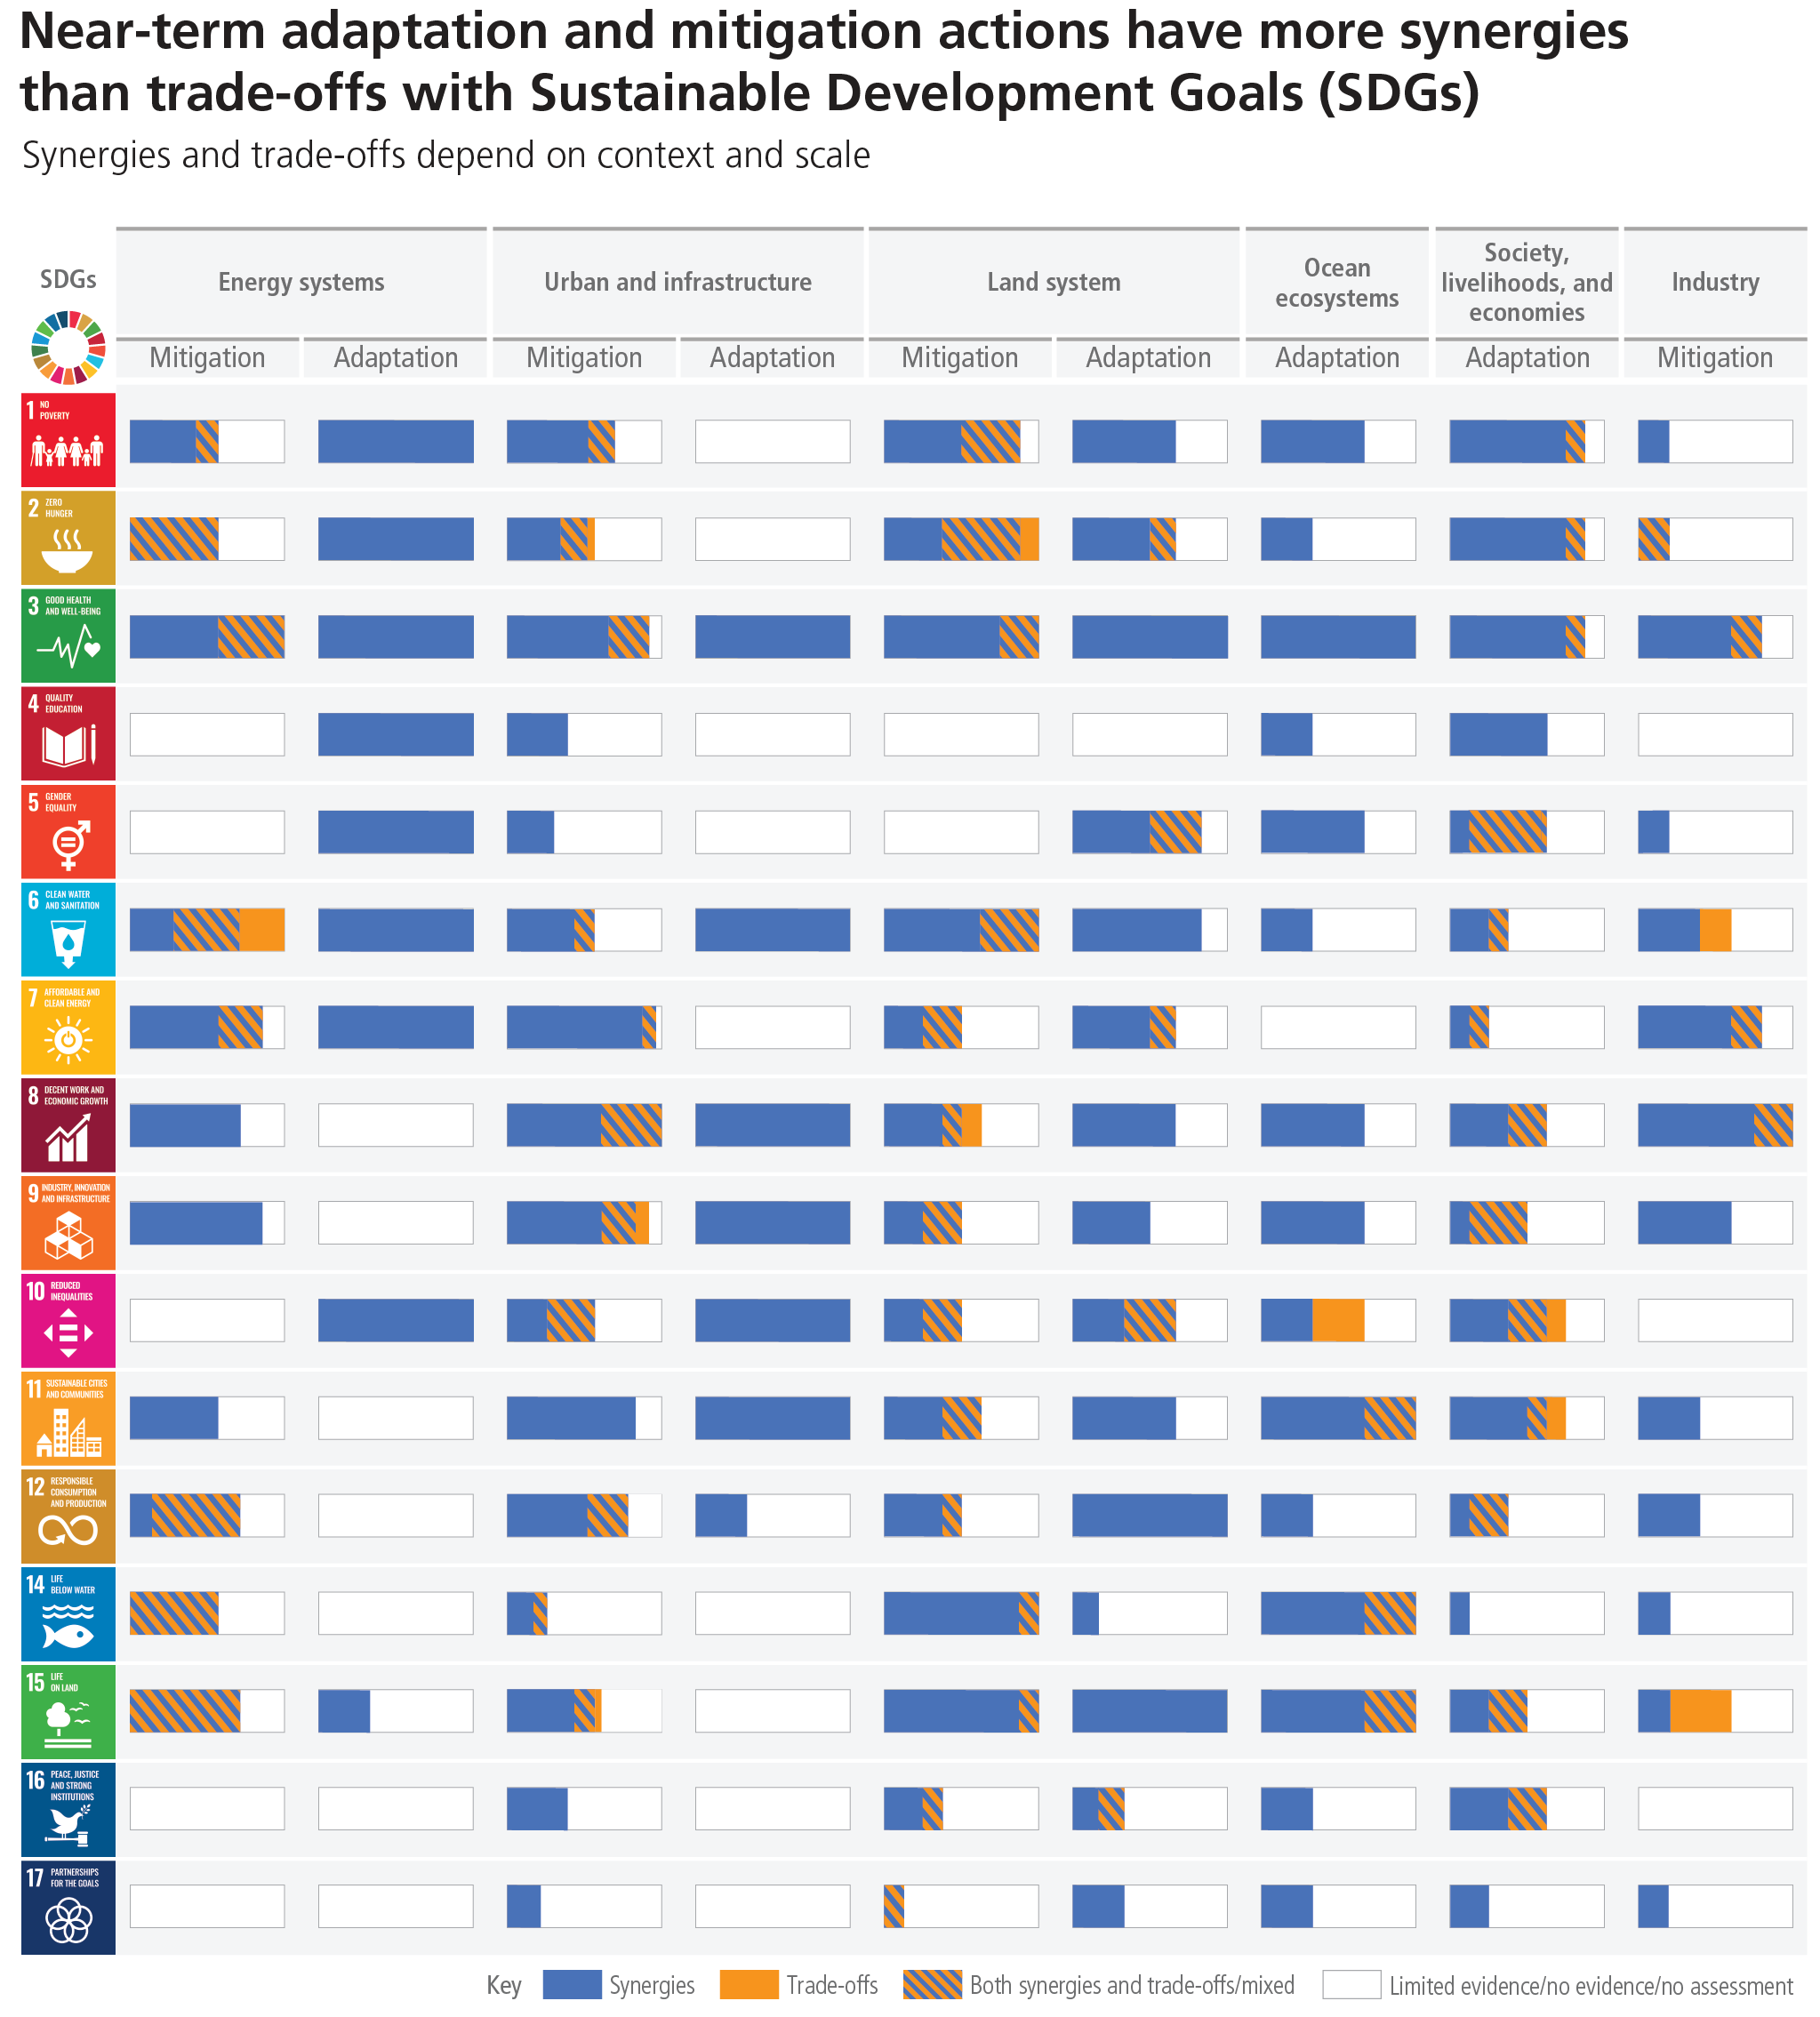
\includegraphics[width=\textwidth]{figs/chap2/IPCC_AR6_SYR_Figure_4_5.png}
    \caption[Synergies and trade-offs of climate action to other SDGs]{Synergies and trade-offs between the portfolio of climate change mitigation and adaptation options and the SDGs \citep{lee2023climate}}
    \label{fig:chap2_fig6}
\end{figure}

On the contrary, trade-offs may emerge if ambitious climate change mitigation aligned with a 1.5°C target alters land use in ways detrimental to sustainable development. For instance, converting natural forests, agricultural areas, or lands under indigenous or local ownership to plantations for bioenergy production could threaten food and water security, lead to conflicts over land rights, and cause biodiversity loss. Additionally, trade-offs may arise in some regions if transitioning from fossil fuels to alternative energy sources lacks careful planning, impacting existing assets, workers, and infrastructure. Effective management can minimize these trade-offs, such as improving bioenergy crop yields to reduce harmful land-use changes or providing retraining opportunities for workers transitioning to lower carbon sectors. \par



